\documentclass[12 pt, a4paper]{article}
\usepackage[norsk]{babel}  								% For norsk oppsett
\usepackage[utf8]{inputenc}
\usepackage{amsmath}
\usepackage{amssymb}
\usepackage{graphicx}
\usepackage{tabularx}
\usepackage{subcaption}
\usepackage{hyperref}
\usepackage{fancyhdr}
\usepackage{enumerate}
\usepackage{float}
\usepackage{tikz}
\usepackage{fancyhdr}
\usepackage{lastpage}
\usepackage{circuitikz}
\usepackage{physics}
\usepackage[includeheadfoot, margin =0.5 in]{geometry}
\usepackage[FYS, OnlyFrontpage]{mnfrontpage} 			%SKIFT HER!!!
\usepackage[version=3]{mhchem}
\usepackage{biblatex}%,style=numeric-comp
%\usepackage{cite}
\usepackage{siunitx}
\usepackage{todonotes}
\usepackage{xcolor}
\usepackage{listings}
\lstset{basicstyle=\ttfamily,
  showstringspaces=false,
  commentstyle=\color{red},
  keywordstyle=\color{blue}
}
%\usepackage{showframe}  %Dette viser hvordan strukturen på sidene er

\setlength{\parindent}{0cm}

\author{
Erik Skaar\\ 
Mikael Kiste\\
Thomas Storaas
}



\bibliography{kilder.bib}






\title{Solarsystem FYS3150/FYS4150}
\begin{document}
\mnfrontpage
\pagebreak



\pagestyle{fancy}
\fancyhf{}
\rhead{FYS3150/FYS4150}
\lhead{Erik Skaar,Thomas Storaas \& Mikael Kiste}
\fancyfoot[CE,LO]{\leftmark}
\fancyfoot[LE,RO]{Page \number\value{page} of \pageref{LastPage}}

\renewcommand{\headrulewidth}{2pt}
\renewcommand{\footrulewidth}{1pt}

\tableofcontents

\marginparwidth = 0.9in

\section*{Abstract}%1
In this report we test the Verlet-Velocity and the Forward-Euler method against each other. Here Verlet-Velocity will come out as a clear winner with an almost equal timing as Forward-Euler and with conserved values for kinetic energy, potential energy, momentum and angular momentum. The Verlet-Velocity is then used for calculations of various solar systems. All calculations are done in 3D, but all the figures are made in 2D. This is to maximize the visual quality of the report. The escape velocity is confirmed and Jupiters mass effect on earth orbit in the three body system is discussed. The Verlet-Velocity fails to produce stable results for this system. The effect of general relativity is confirmed through a simulation of the perihelion precession of Mercury. 



\pagebreak
\section{Introduction}
For thousand of years humankind have looked up to the beyond and wondered. Specifically our race has wondered about the motion of our solar system. Finally after Newton the mystery was solved. Newton developed the gravitational law, which made it possible to predict the motion of the planets. After a couple of centuries Einstein came with the thoery of general relativity and made a small refinement to the law of motion that Newton proposed. 
\\
\\
These laws are not enough to solve the motion of the planets. The laws makes differential equation which are not trivial or even impossible to solve. This is where a our computational physics course comes in \todo{REF KURSETS HJEMMESIDE}. With the tools developed in this course we can make a prediction to the motion of the planets in our solarsystem. 
\\
\\
In this project we will make an object oriented code to solve the solar system with Forward Eulers method and Velocity Verlet. Both method will be derived, discussed, implemented and benchmarked for the Earth-Sun system. 
\todo{WRITE ABOUT THEIR PERFORMANCE}
\\
\\
Finally, a relativistic correction was made....... 
\todo{NEED TO IMPLEMENT THIS AND GET FACTS}


\section{Theory}
\subsection{Gravitation}

We will simulate the solar system with only the gravitational force affecting the planets.  Newton's gravitational law is stated in equation (\ref{eq:newton}). Where G is the gravitational constant ($6.67 \cdot 10^{-11} \rm{Nm^2/s^2}$), r is the distance between the planets, m is the mass of the object and M is the mass of the other object.

\begin{align}
	\vec{F_G}  =\frac{GmM}{\vec{|r|}^3}\vec{r}
	\label{eq:newton}
\end{align}

Thankfully for us the force is an attractive force. It is worth noting that if the sun is at origo distance is simply the norm position vector of the planet. From now on we will denoted the different masses with $M_{planet name}$ except for the sun that has the special symbol $M_{\odot}$. 
\\
\\
If you have n object attracting each other the total gravitational force, $F_k$, for each object is: 


\begin{align}
	F_k = 
	\sum_{i = 1}^{N}
	\vec{F_i}  
	=
	\frac{Gm_km_i}
	{\vec{|r_k - r_i|}^3}
	(\vec{r_k} - \vec{r_i})
	(1 - \delta_{k,i})
	\label{eq:newton_all}
\end{align}

Where $\delta_{k,i}$ is the function:

\begin{align*}
	\delta_{k,i} = \left\{\begin{matrix}
					1 & \text{if} \quad k =  i\\
					0 & \text{if} \quad k \neq i 
					\end{matrix}\right.
\end{align*}



We can use Newton's second law to determine the accelration of the planet. Newton's second law state $F = m\vec{a}$. Which translate to:

\begin{align}
	a_k
	=
	\sum_{i = 1}^{N}
	\frac{Gm_i}
	{|\vec{r_k} - \vec{r_i}|^3}
	(\vec{r_k} - \vec{r_i})
	(1 - \delta_{k,i})
	\label{eq:acceleration_all}
\end{align}



\subsection{Units}
As a famous person once said, \"If you use seconds and meters you will not finish within the deadline\". I think our professor, Morten Hjorth-Jensen, is on to something. Seconds and meters are impractical in this project. Therefore we use more suitable units. The distance between the earth and sun, 149 597 870 691 meter, is defined as one astronomical unit (au). For time one year seems reasonable. 
These are the units that will be used in this project. 
\\
\\
We can now express the gravitational constant with these units. To do this we use the formula for the acceleration for a circular orbit is $\frac{v^2}{r}$. Combine this with the gravitational law, we get: 

\begin{align*}
	\frac{v^2}{r} =
	\frac{GM_{\odot}}{\vec{|r|}^3}\vec{r} 
	\implies 
	G
	=
	\frac{v^2 r}{M_{\odot}} = \frac{\rm{au} (2\pi \cdot \rm{au/year})^2}{M_{\odot}}
	=
	\frac{4\pi^2}
	{M_{\odot}} \rm{au^3/year^2}
\end{align*}

Applying this to equation (\ref{eq:acceleration_all}), we get: 

\begin{align}
	a_k
	=
	\sum_{i = 1}^{N}
	4 \pi \frac{m_i}{M_{\odot}}
	\frac{(\vec{r_k} - \vec{r_i})}
	{|\vec{r_k} - \vec{r_i}|^3}
	(1 - \delta_{k,i}) \rm{au^3/year^2}
	\label{eq:acceleration_all_au}
\end{align}














\subsection{prehelion}


\todo{since this is not implemented in the code yet nothing is writen}
















\subsection{Numerical methods}

Equation (\ref{eq:acceleration_all_au}) initial conditions for velocity and position determines the orbit of the planets. 
These equations are for x,y,z direction and when writen out you get a coupled set of differential equations. This set is near impossible to solve analytically. It might be impossible. We will use numerical methods to solve this set. More specifically we will use the Forward Euler method and the Velocity-Verlet method. A given $t_i$ is equal to $t_0 + ih$, where $h = (t_{0} + t_{n})/n $.

\subsubsection{Forward Euler}

Both method use a Taylor polynomial approximation to solve the set of differential equation. The Forward Euler use the first order Taylor polynomial. With $r'(t) = v(t)$ and $v'(t) = a(t)$ the Forward Euler method result in: 
 
\begin{align}
	&\vec{r_i}(t+h) \approx \vec{r_i}(t) + h \vec{v_i}(t)
	\\
	&\vec{v_i}(t+h) \approx \vec{v_i}(t) + h \vec{a}(t)
	\label{eq:euler}
\end{align}

The error for a first order taylor polynomial goes as $\mathcal{O}(h^2)$ \todo{REF TO LECTURE NOTES}. This is the error for each step. The error is accumulated for each step and will thereby be proportional to h. 

\subsubsection{Velocity-Verlet}

You guessed it, this is the second order Taylor polynomial. . As I said the Velocity-Verlet method is based on a Taylor polynomial approximation. And this is the second order. 

\begin{align}
	&\vec{r_i}(t+h) \approx \vec{r_i}(t) + h \vec{v_i}(t) + \frac{1}{2} h^2 a(t)
	\\
	&\vec{v_i}(t+h) \approx \vec{v_i}(t) + h \vec{a}(t) + \frac{1}{2} h^2 \vec{a}'(t)
	\label{eq:verlet}
\end{align}

Since we have no formula for the derivative of a, we use the approximation: 
\todo{ER DET DELT PÅ 2 ELLER h? } 

\begin{align*}
	\vec{a}'(t) \approx \frac{\vec{a}(t+h) - \vec{a}(t)}{h}
\end{align*}

We simply update the position first. We keep the old acceleration and calculate the acceleration at the new position.  Using this equation (\ref{eq:verlet}) we get: 

\begin{align*}
	&\vec{v_i}(t+h) \approx \vec{v_i}(t) + h \vec{a}(t) + \frac{1}{2} h(\vec{a}(t+h) - \vec{a}(t))
	\\
	&\vec{v_i}(t+h) \approx \vec{v_i}(t) + \frac{1}{2} h(\vec{a}(t+h) + \vec{a}(t))
\end{align*}

The error for a first order taylor polynomial goes as $\mathcal{O}(h^2)$ \todo{REF TO LECTURE NOTES}. This is the error for each step. The error is accumulated for each step and will thereby be proportional to $h^2$. This is one order of magnitude better, then the Forward Euler method. 




















\section{Method}
\subsection{Implementation of code}

The implementation is writen in c++ and is object oriented. We found it natural to divide the project in to two classes and one main program. 
\\
\\
We made one class for the planet (\href{https://github.com/erikfsk/Project-3/blob/master/Project3/planet.cpp}{\textcolor{blue}{planet.cpp}} and \href{https://github.com/erikfsk/Project-3/blob/master/Project3/planet.h}{\textcolor{blue}{planet.h}}). This class contain variables for the position, velocity, mass for the specific planet and a specific filename. The class has methods for updating position, velocity and acceleration as outlined in section \ref{sec:theory}. Also methods for writing to a file was implemented. 
\\
\\
The second class is for the solarsystem (\href{https://github.com/erikfsk/Project-3/blob/master/Project3/solarsystem.cpp}{\textcolor{blue}{solarsystem.cpp}} and \href{https://github.com/erikfsk/Project-3/blob/master/Project3/solarsystem.h}{\textcolor{blue}{solsystem.h}}). The solar system contain a list with all the planets and has methods to make the planets move and react to each other. You can look at the solar system as a class with for-loops for the planets. 
\\
\\
The \href{https://github.com/erikfsk/Project-3/blob/master/Project3/main.cpp}{\textcolor{blue}{main.cpp}} program is where all the inputs to the solar system is given. Here all the initial condition for the planets are stated and organized for proper input to the solarsystem class.
\\
\\
All these programs are combined with \href{https://github.com/erikfsk/Project-3/blob/master/Project3/makefile}{\textcolor{blue}{makefile}}. When this is done the \href{https://github.com/erikfsk/Project-3/blob/master/Project3/solsys.exe}{\textcolor{blue}{solsys.exe}} will be made. Takes in three arguments. The first argument is the number of planets that you would like to simulate. This is a preset list of the bodies in the solarsystem. Where the Sun is the first element, Earth is the second and Jupiter is the third. After that they ascend based on radius. The second argument is the end time measured in years from now. The start time is set to 19th of october 2017. This is the time that the intial values were obtained from \href{https://ssd.jpl.nasa.gov/horizons.cgi#top}{\textcolor{blue}{NASA}}. Finally the third argument is the number of steps, n. 
\\
\\
Finally, in our github repository there is directories were earlier versions can be found. For instance the 
\href{https://github.com/erikfsk/Project-3/tree/master/Project3/}{\textcolor{blue}{Project3}} directory is for where all the code is centered. In this directory there are many directories with different results files and python scripts for making figures. There are also a coupled of other main.cpp variants. These are for different assignments in this project. It should be pretty self ex<planet>ory. 


\subsection{FLOPs for the algorithms}\label{sec:flops}

The counting of the FLOPs are in the section \ref{sec:appendix}, a.k.a. appendix. There we show sudo-code. For each line of code there is a corresponding comment that counts flops. For each method there is a header comment explaining what method and algorithm it represent. After each method there is a final comment with total FLOPs.
\\
\\
Common for both algorithms are calculation of the acceleration. The acceleration itself is 19 FLOPs. But for both algorithm this is called $n(n-1)$ times. After that the Forward Euler method calls functions to set position and velocity. This is done for all the planets. And for each planet it costs 6 FLOPs for the position and 6 more for the velocity. This gives a total of:

\begin{align*}
	19n(n-1) + 12n = 19n^2 - 7n
\end{align*}

For the Verlet-Velocity it is 21 FLOPs for the position and 12 FLOPs for the velocity (nothing is precalculated). This is of course done for all the planets and give us: 

\begin{align*}
	19n(n-1) + 33n = 19n^2 + 14n
\end{align*}
%((19*(9^2) + 14*9)- (19*(9^2) - 7*9)) /(19*(9^2) -7*9)
So, this means that for 9 planets the verlet method has about 10 \% more FLOPs, which is not much considering that much of the time are used on writing to file and getting variables and so on. The difference between the two algorithms should not be much.






























\section{Result \& Discussion}











\subsection{Earth-Sun system}








\subsubsection{Stability}

\begin{figure}[H]
    \centering
    \begin{subfigure}{0.5\textwidth}
        \centering
        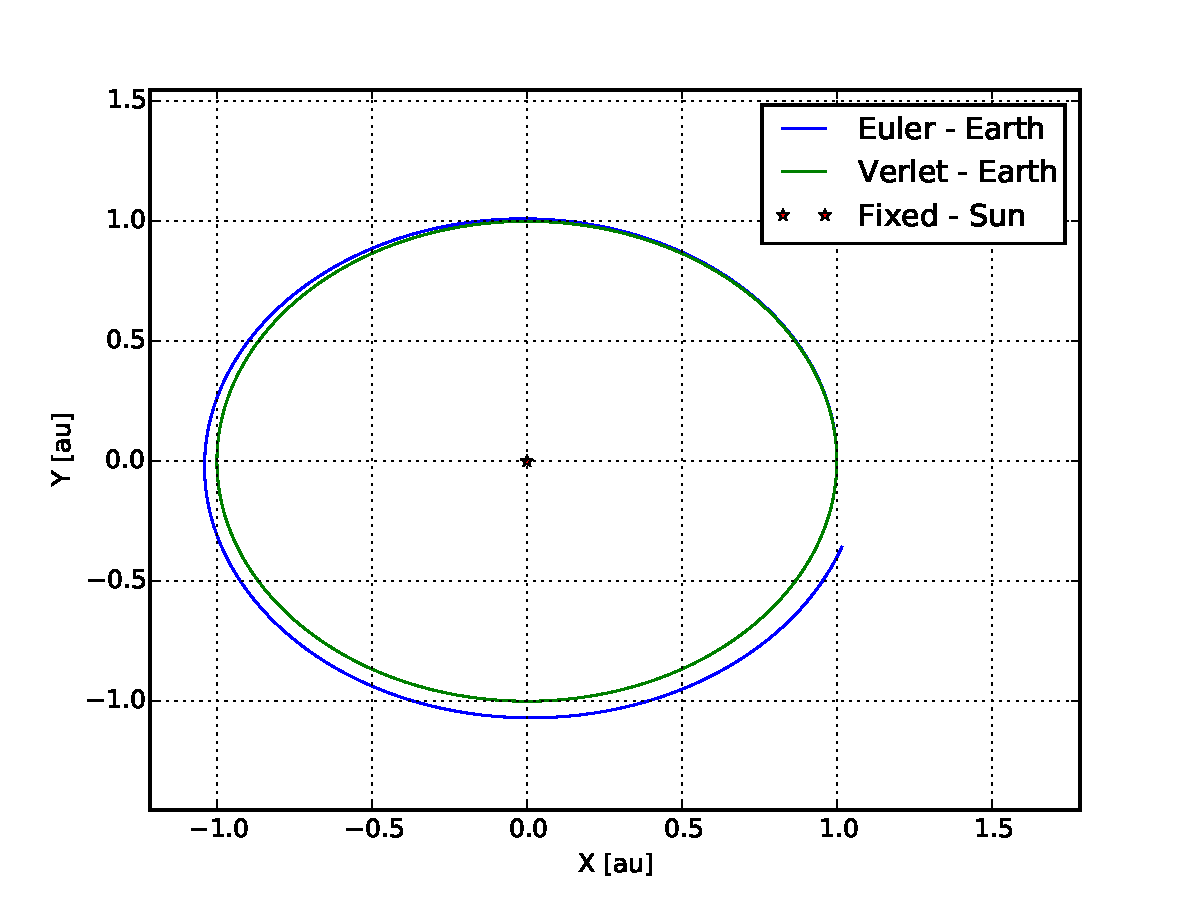
\includegraphics[width=\linewidth]{result/bilder/earth-sun.pdf}
    	\caption{}
    \end{subfigure}%
    ~ 
    \begin{subfigure}{0.5\textwidth}
        \centering
        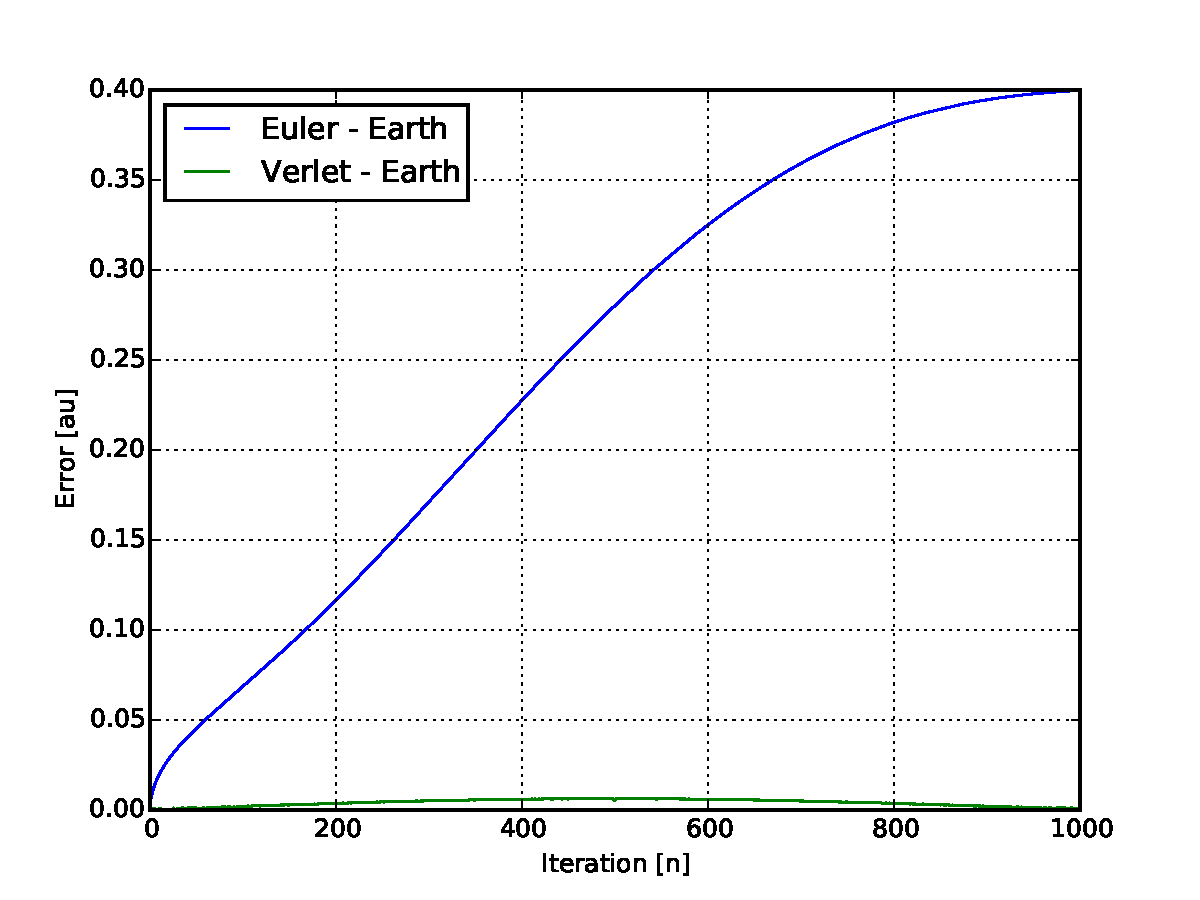
\includegraphics[width=\linewidth]{result/bilder/earth-sun-error.pdf}
        \caption{}
    \end{subfigure}
    \caption{a) show the orbit of earth around the sound. The intial velocity is set to $2\pi$ in y direction and the start position to 1 au in x direction. b) shows how the error behaves. The intial values should give a perfect circular motion. So the error is calculated by $r_i - r_{0}$. It is clear that Verlet-Velocity method is superior. This simulation was with 1000 points with the end time of 1 year. Both simulations was produced by \href{https://github.com/erikfsk/Project-3/blob/master/Project3/3a/plot_earth_sun.py}{\textcolor{blue}{plot\_earth\_sun.py}}}
    \label{fig:earth-sun}
\end{figure}


\begin{center}
\label{table:euler-verlet-time}
\captionof{table}{Time table for the different algorithms. The algorithms use nearly the same time. This is not a shocker since the number of FLOPs for the algorithms are similar, see section (\ref{sec:flops}). Disclaimer: this is only the result from one test, but several was done. Both algorithms were very close and it seem to be random which is fastest.
\\}
\begin{tabular}{c c c c c}
    \hline 
    \hline 
    n & Forward-Euler & Verlet-Velocity &  fastest & $\frac{slowest}{fastest}$\\ 
    \hline
    10 & 0.000136 & 0.000148 & Euler &   1.08823529412   \\ 
    100 & 0.000208 & 0.000179 & Verlet &   1.16201117318   \\ 
    1000 & 0.000392 & 0.000389 & Verlet &  1.00771208226   \\ 
    10000 & 0.002427 & 0.002426 & Verlet &   1.00041220115  \\ 
    100000 & 0.022931 & 0.022293 & Verlet &   1.02861884897   \\ 
    1000000 & 0.167022 & 0.175944 & Euler &   1.05341811258  \\ 
    10000000 & 1.58721 & 1.52666 & Verlet &   1.03966174525  \\ 
    100000000 & 15.1786 & 15.1176 & Verlet &   1.00403503202  \\ 
    \hline
\end{tabular}
\end{center}














\subsubsection{Conserved quantities}

All the figures in this section was made from the data and python script in the directory \href{https://github.com/erikfsk/Project-3/tree/master/Project3/conserved-values}{\textcolor{blue}{conserved-values}}.

\begin{figure}[H]
    \centering
    \begin{subfigure}{0.5\textwidth}
        \centering
        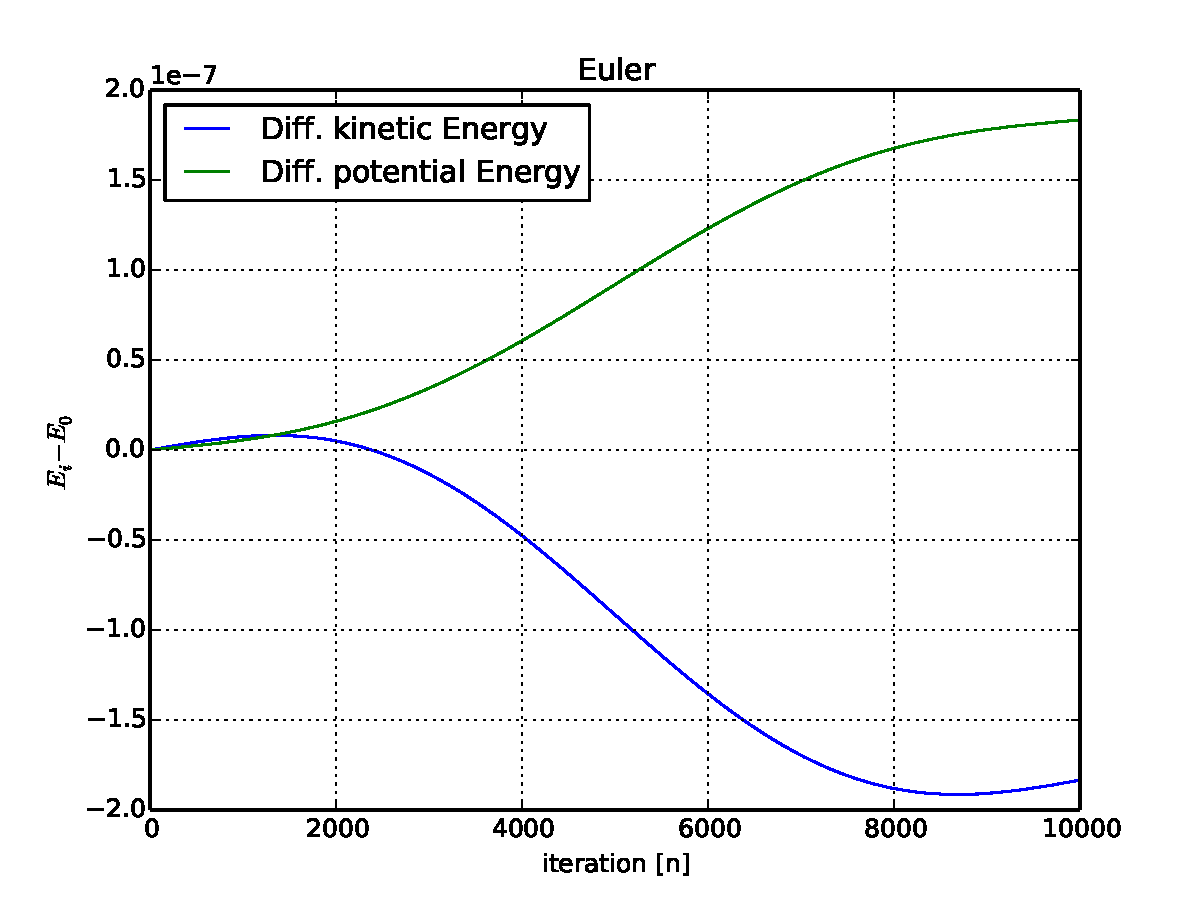
\includegraphics[width=\linewidth]{result/bilder/kin-pot-euler.pdf}
    	\caption{}
    \end{subfigure}%
    ~ 
    \begin{subfigure}{0.5\textwidth}
        \centering
        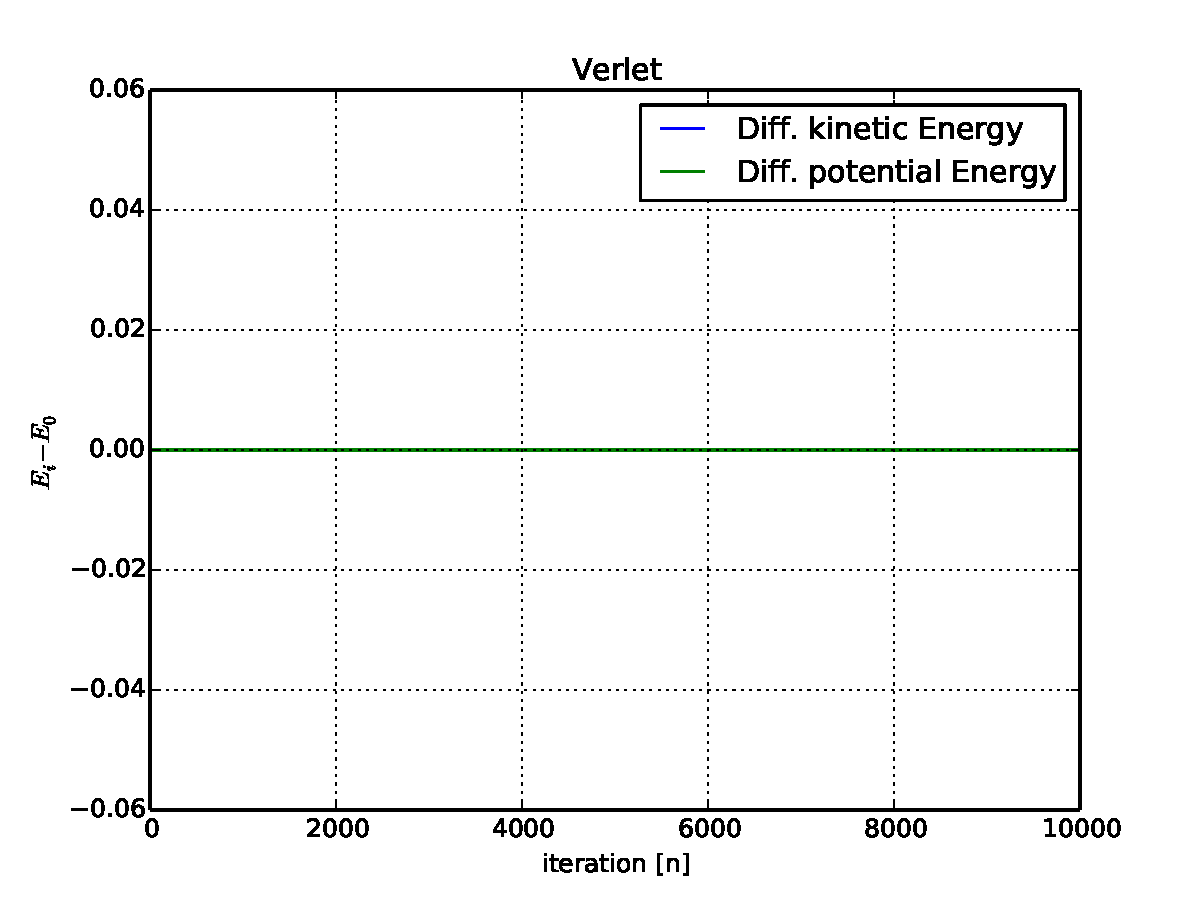
\includegraphics[width=\linewidth]{result/bilder/kin-pot-verlet.pdf}
        \caption{}
    \end{subfigure}
    \caption{Both are figures are graphs of the kinetic energy and potential energy and how it differ from they intial value. a) is the Forward Euler method and b) is the Verlet-Velocity method. As expected the energies are not conserved in the Forward Euler method, but is conserved in the Verlet-Velocity.}
    \label{fig:conserved-energy}
\end{figure}





\begin{figure}[H]
    \centering
    \begin{subfigure}{0.5\textwidth}
        \centering
        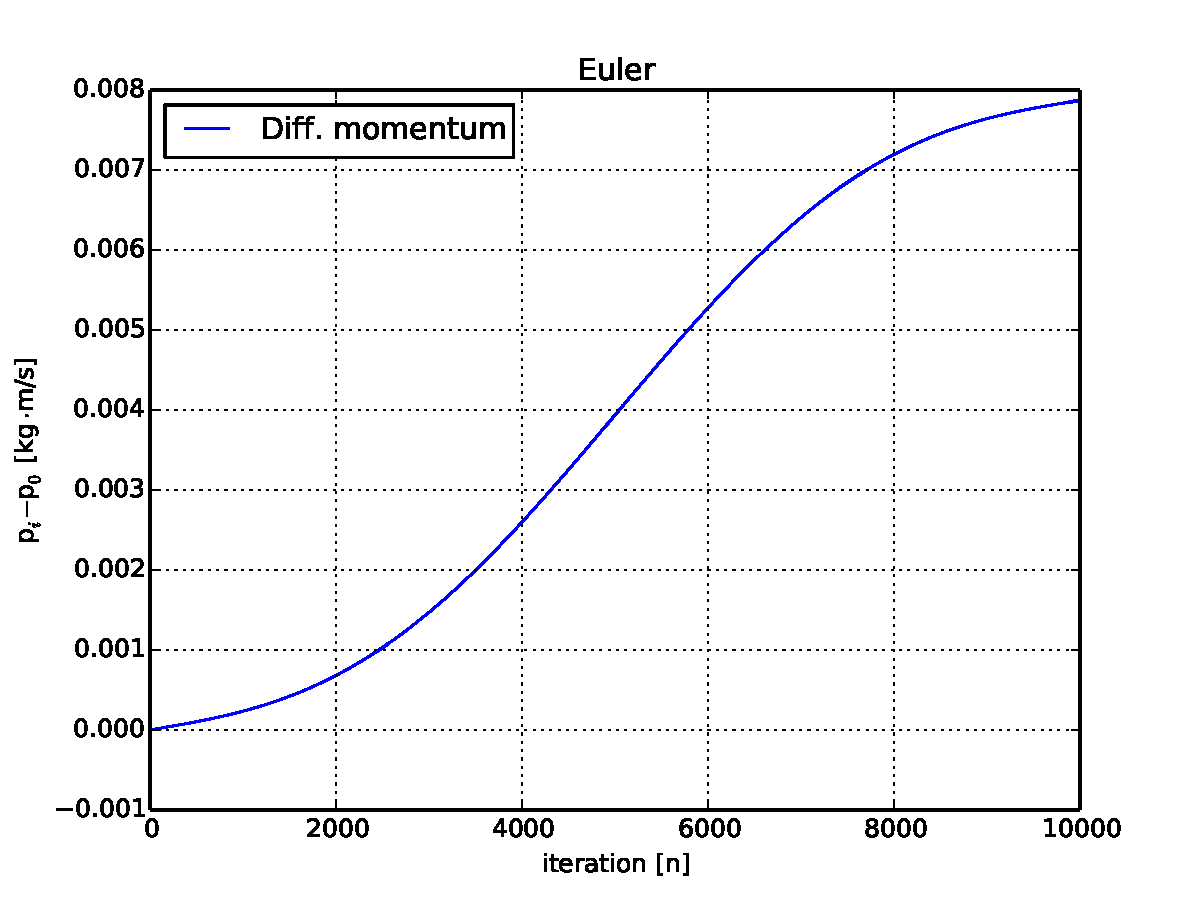
\includegraphics[width=\linewidth]{result/bilder/momentum-euler.pdf}
    	\caption{}
    \end{subfigure}%
    ~ 
    \begin{subfigure}{0.5\textwidth}
        \centering
        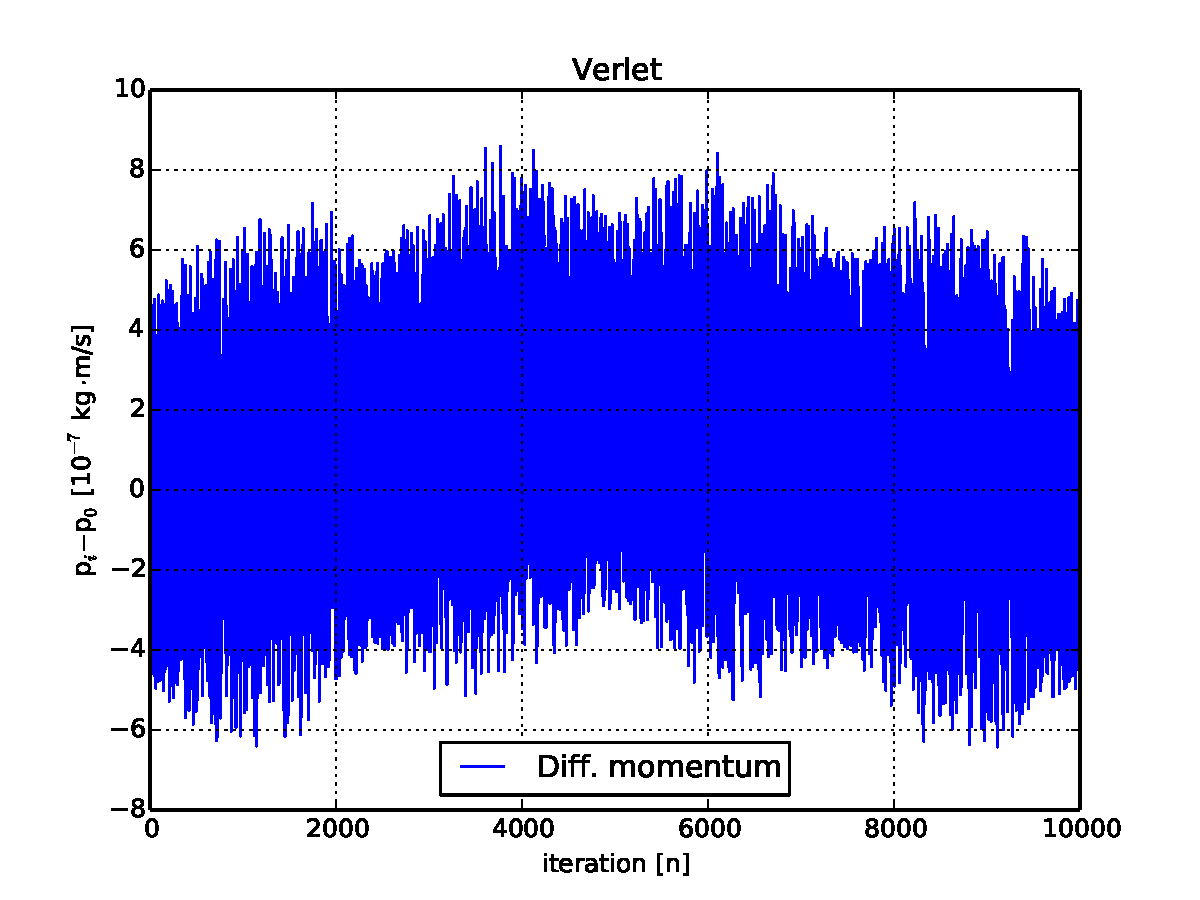
\includegraphics[width=\linewidth]{result/bilder/momentum-verlet.pdf}
        \caption{}
    \end{subfigure}
    \caption{Both are figures are graphs of the momentum and how it differ from they intial value. a) is the Forward Euler method and b) is the Verlet-Velocity method. It should come as no suprise that momentum is not conserved for the Forward Euler method as the kinetic energy was not conserved, as the mass is a constant. Once again the Verlet-velocity method conserve the quantity. 
    }
    \label{fig:conserved-momentum}
\end{figure}





\begin{figure}[H]
    \centering
    \begin{subfigure}{0.5\textwidth}
        \centering
        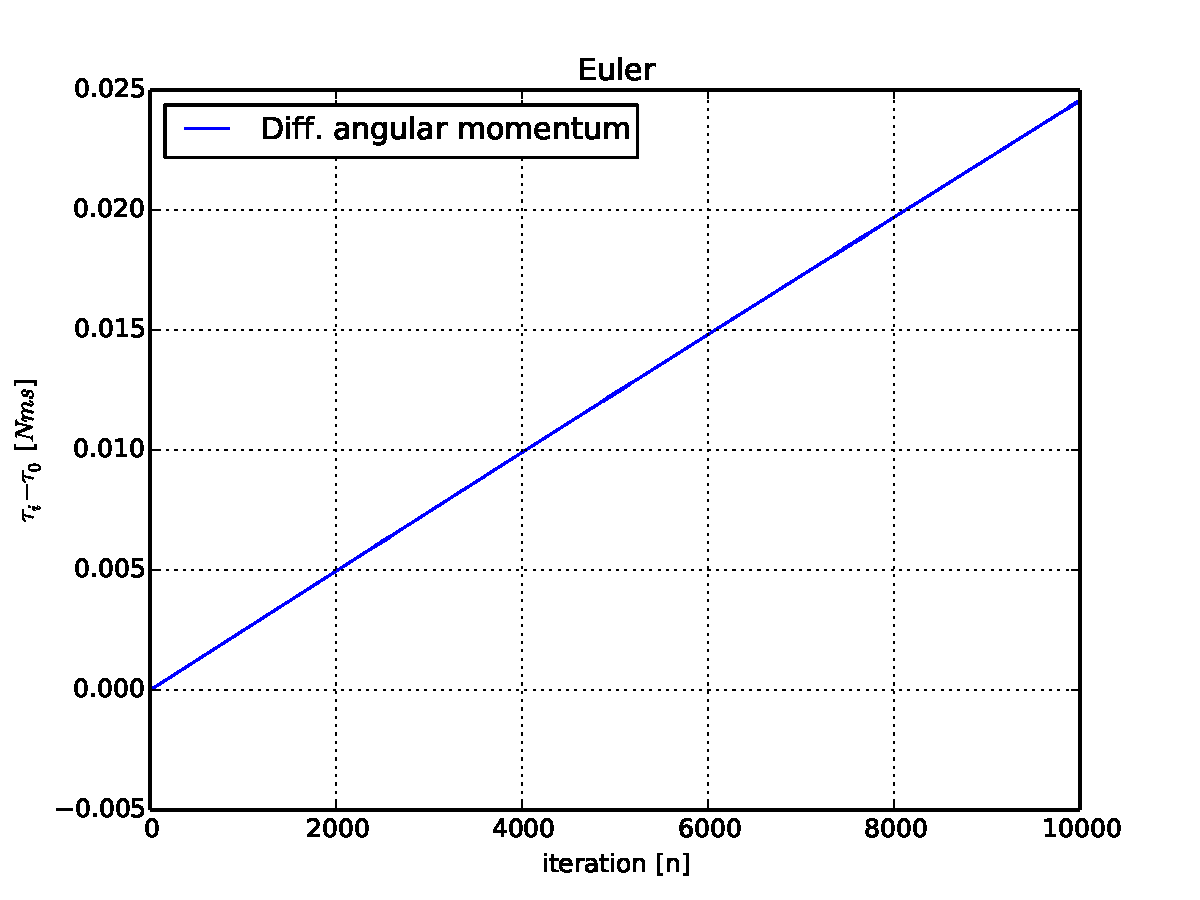
\includegraphics[width=\linewidth]{result/bilder/ang-momentum-euler.pdf}
        \caption{}
    \end{subfigure}%
    ~ 
    \begin{subfigure}{0.5\textwidth}
        \centering
        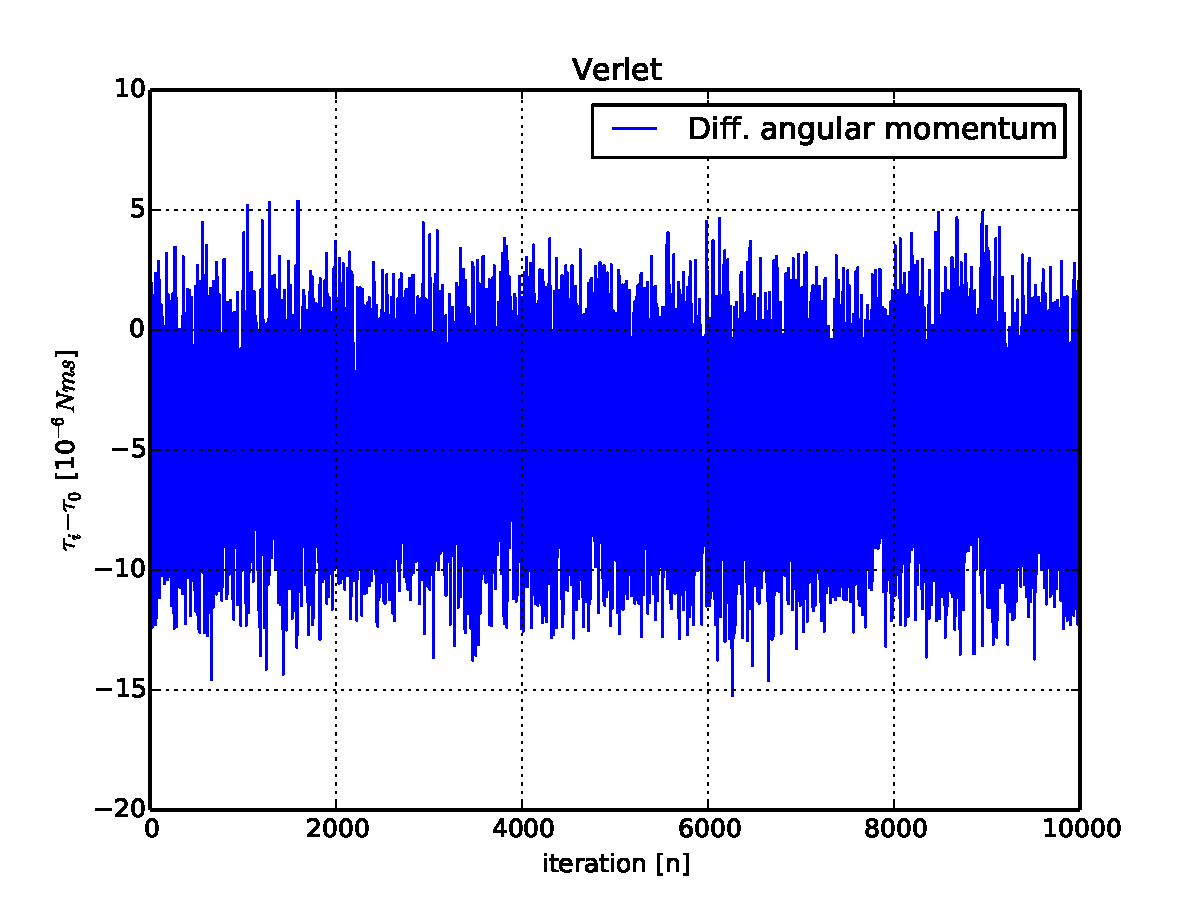
\includegraphics[width=\linewidth]{result/bilder/ang-momentum-verlet.pdf}
        \caption{}
    \end{subfigure}
    \caption{Both are figures are graphs of the angular momentum and how it differ from they intial value. a) is the Forward Euler method and b) is the Verlet-Velocity method. Forward Euler is once again not capable of conserving the value, but luckily for us the Verlet-Velocity method is. 
    }
    \label{fig:conserved-ang}
\end{figure}















\subsubsection{Escape velocity}

The assignment was to find the escape velocity for the earth by trial and error. Fortunate for us that we know some math and can calculate it. See section \ref{sec:escape-velocity} for this. But we started guessing \"randomly\" (winking Face emoji). Figure (\ref{fig:escape-velocity-low}) a) shows these guesses. Where we can see that the velocities around 8.8 au/year shots out and never returns. 
The algorithms only runs for 15 years and will thereby not see the 8.8 au/year return to orbit even tho it should. The plots were made by the data and python scripts in the directory \href{https://github.com/erikfsk/Project-3/tree/master/Project3/escape-velocity}{\textcolor{blue}{escape-velocity}}.

\begin{figure}[H]
    \centering
    \begin{subfigure}{0.5\textwidth}
        \centering
        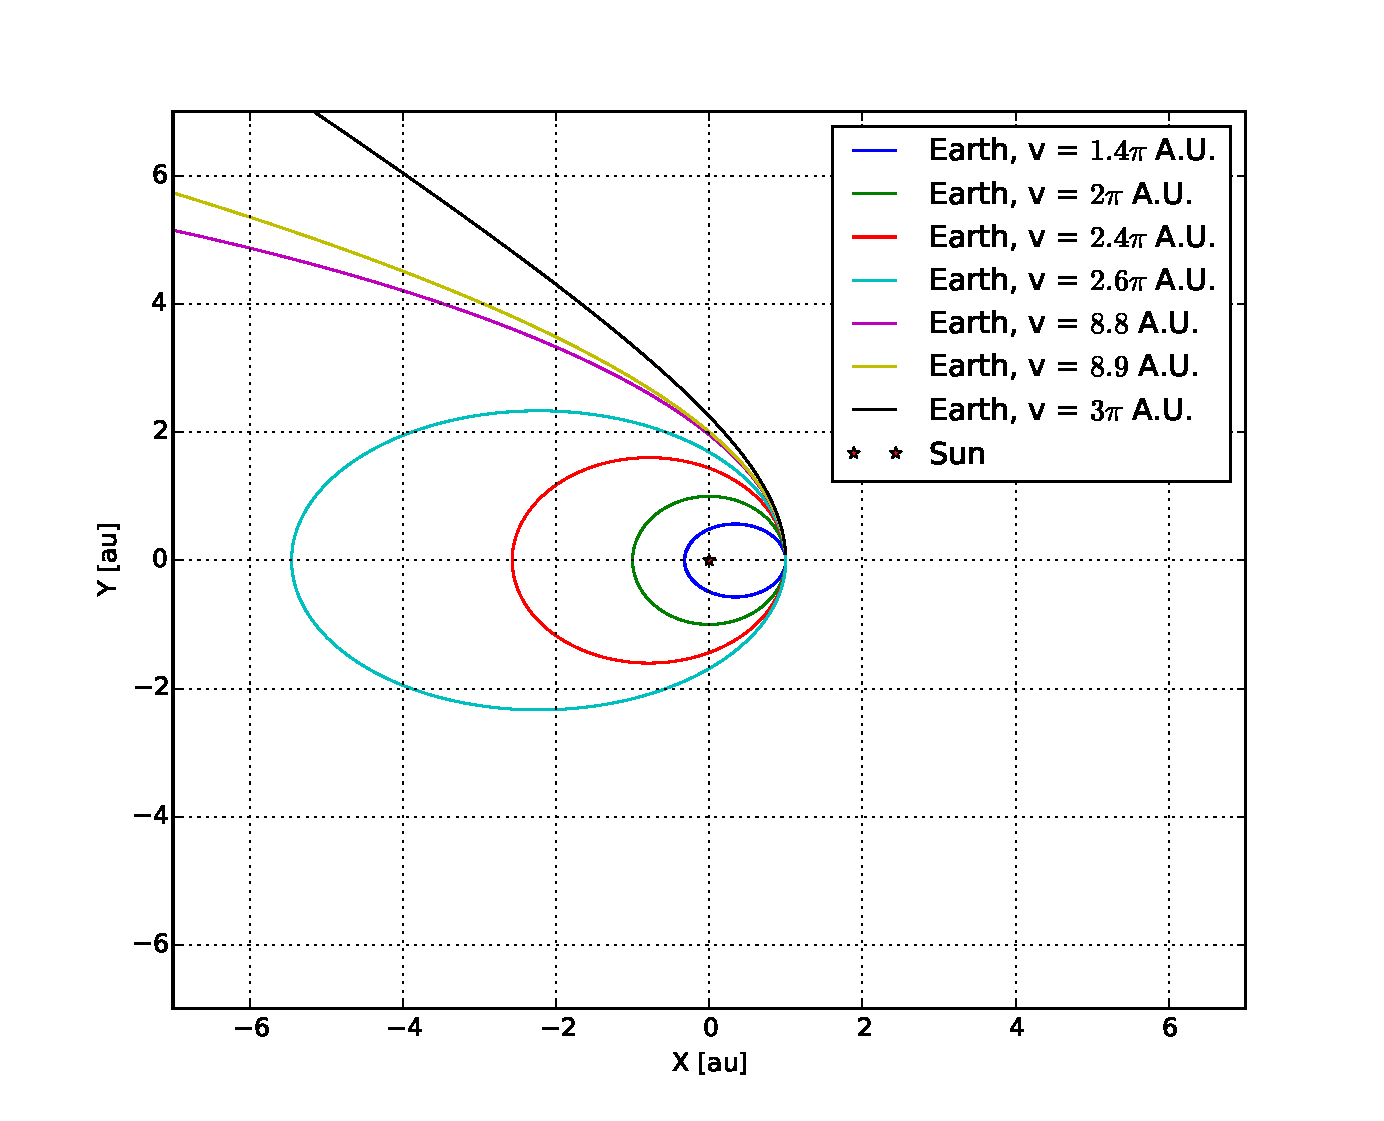
\includegraphics[width=\linewidth]{result/bilder/escape-velocity.pdf}
    	\caption{}
    \end{subfigure}%
    ~ 
    \begin{subfigure}{0.5\textwidth}
        \centering
        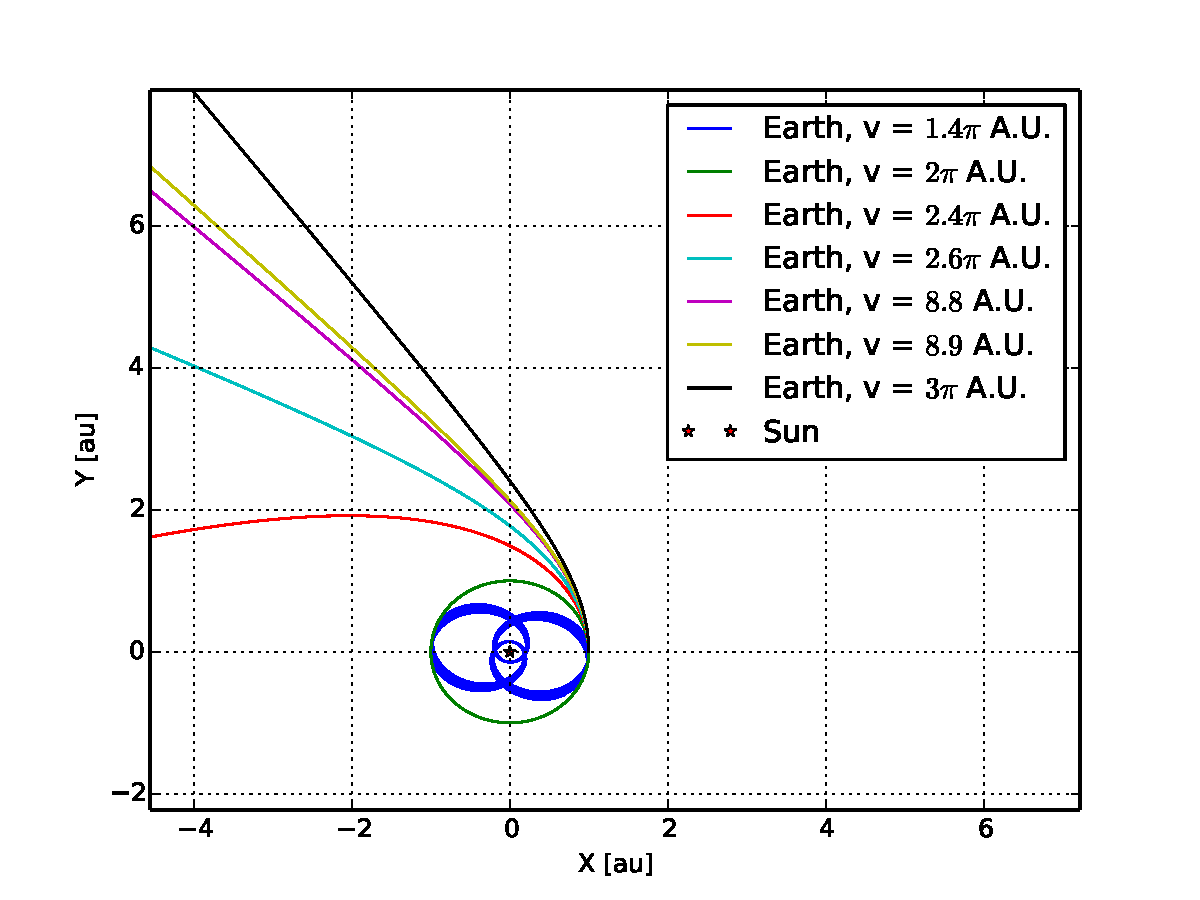
\includegraphics[width=\linewidth]{result/bilder/escape-velocity-r25.pdf}
        \caption{}
    \end{subfigure}
    \caption{a) Show how the orbits of earths with different initial velocity are. b) Shows the same as a) but this time the dependency of r in the denominator in equation (\ref{eq:newton}) is set to 3.5.}
    \label{fig:escape-velocity-low}
\end{figure}



\begin{figure}[H]
    \centering
    \begin{subfigure}{0.5\textwidth}
        \centering
        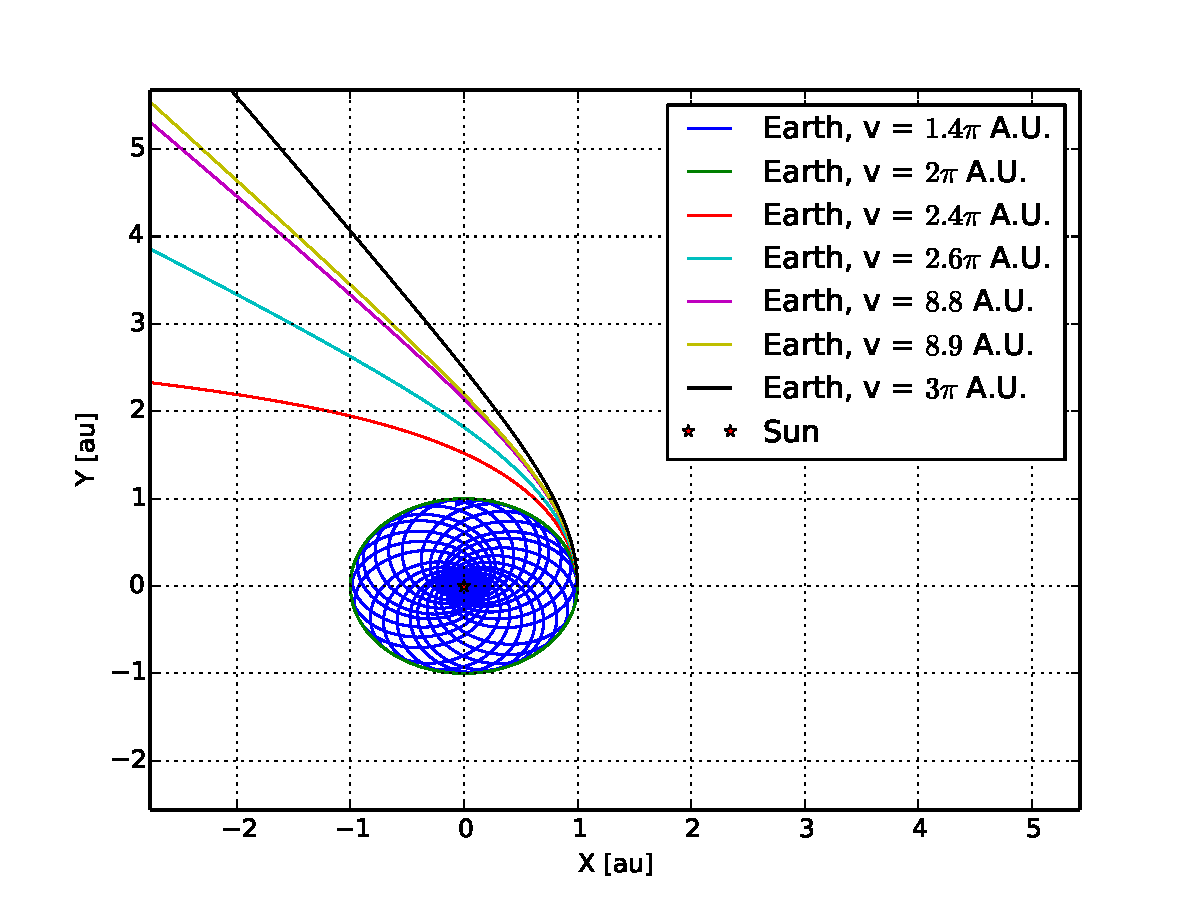
\includegraphics[width=\linewidth]{result/bilder/escape-velocity-r275.pdf}
    	\caption{}
    \end{subfigure}%
    ~ 
    \begin{subfigure}{0.5\textwidth}
        \centering
        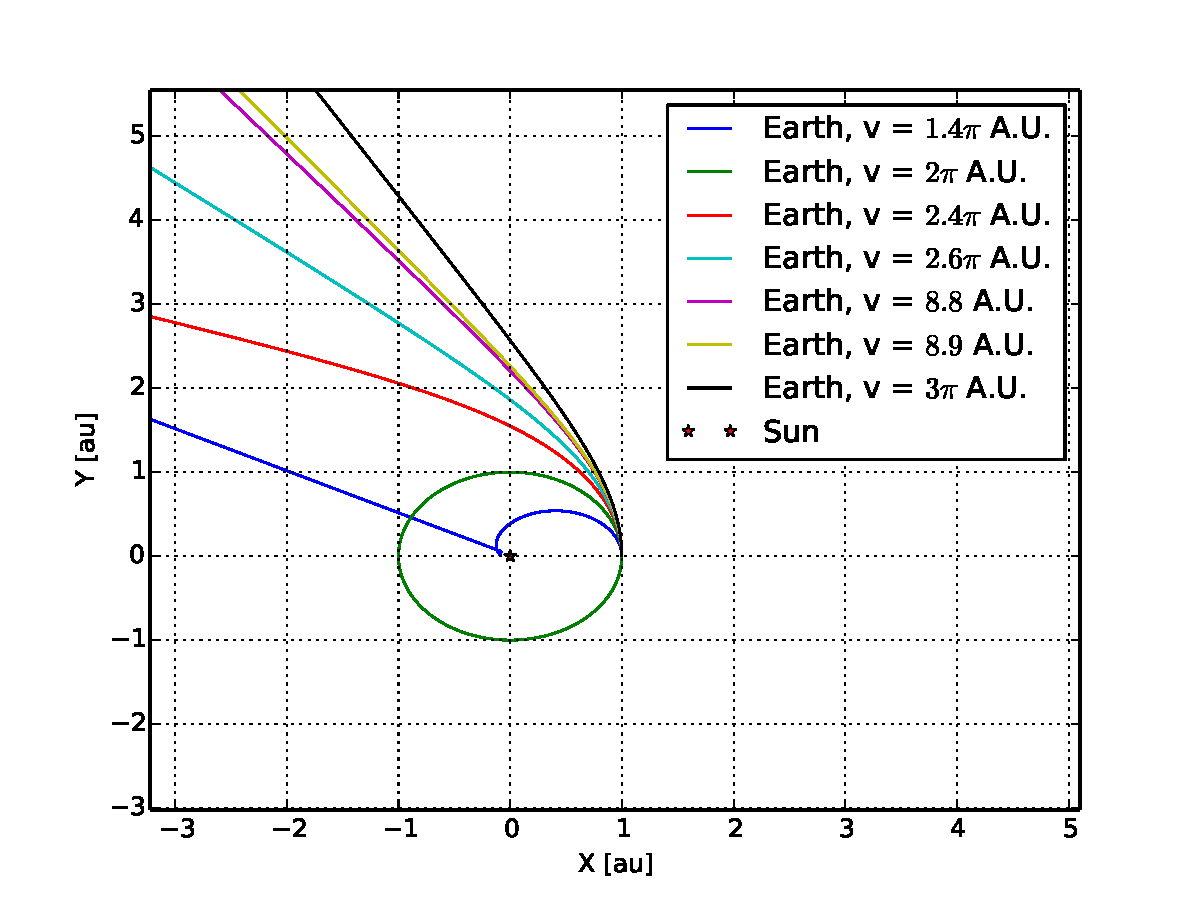
\includegraphics[width=\linewidth]{result/bilder/escape-velocity-r3.pdf}
        \caption{}
    \end{subfigure}
    \caption{a) Shows the same as figure (\ref{fig:escape-velocity-low}) but this time the dependency of r in the denominator in equation (\ref{eq:newton}) is set to 3.75. b) Shows the same as a) but this time the dependency of r in the denominator in equation (\ref{eq:newton}) is set to 4. }
    \label{fig:escape-velocity-high}
\end{figure}


Personally I feel extremly lucky for living in a universe with a r dependency of 2, but then again i probably would not exist if the dependency was different. All the other dependencies are very unstable for even the slightest change in velocity from a perfect circle.


















\subsection{Three body system}

All the figures in this section has been made from the directory \href{https://github.com/erikfsk/Project-3/tree/master/Project3/mass%20jupitur}{\textcolor{blue}{mass jupitur}}. In this directory there are different directories for the r dependency and a python script to generate graphs. The assignment said to try with mass multiplied with 10 and 1000. It was fun, so we did 10,100,1000 and 1100. Hope you enjoy the results. 

\subsubsection{Fixed mass for jupitur}

For a simulation with jupitur original mass 100000 points over 15 years is sufficient to calculate the orbits of the planets. The figure (\ref{fig:three-body}) is quit smooth and you should not expect to get any major change in the result even with many more points per year. 

\begin{figure}[H]
    \centering
    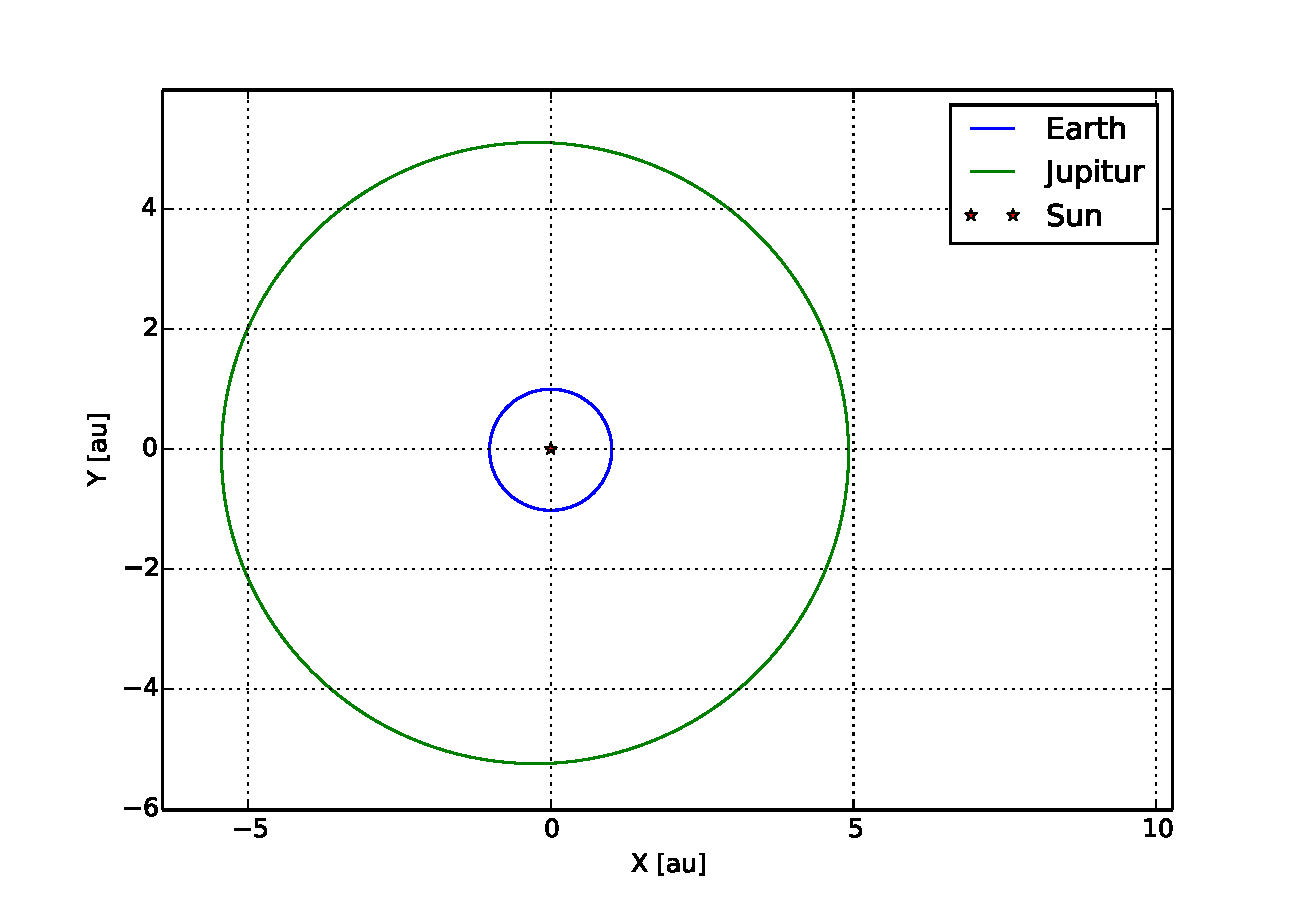
\includegraphics[width=\linewidth]{result/bilder/jupitur-mass.pdf}
    \caption{Plot of the three body system with Earth, Jupitur and the sun. The graph is discussed in the paragraph above. }
    \label{fig:three-body}
\end{figure}


\subsubsection{Varying mass for jupitur}

For varying mass it is mostly the same as for the original mass. For the mass multiplied with 10 and 100 the orbit is \"normal\" with some slight changes and you should not expect any major differences with higher amount of points per year. For the biggest masses the results vary much more on the number of steps per year. I found a couple of hundred thousand steps in total gave a good approximation. A bit higher step count makes earth disappear and a way bigger step count makes the earth come back to orbit like shown below. This is basicly the best of both worlds. The graphs is few point, so easy for python to plot, and has a pretty good approximation.

\begin{figure}[H]
    \centering
    \begin{subfigure}{0.5\textwidth}
        \centering
        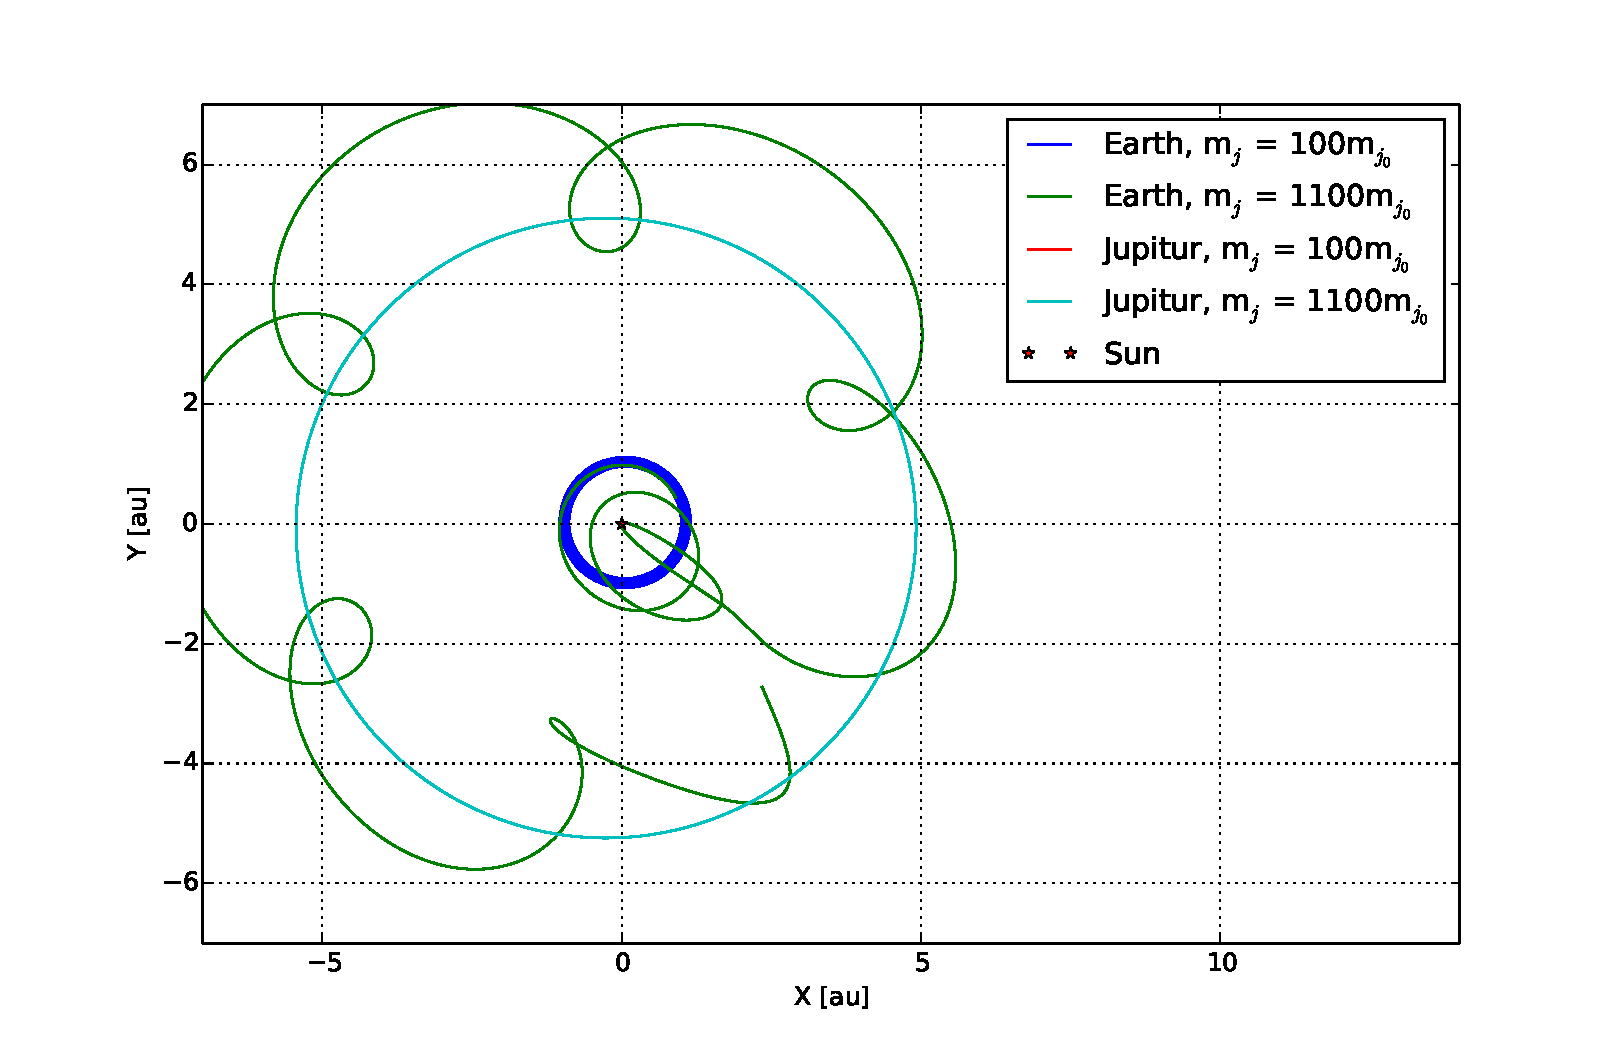
\includegraphics[width=\linewidth]{result/bilder/jupitur-mass-three.pdf}
    	\caption{}
    \end{subfigure}%
    ~ 
    \begin{subfigure}{0.5\textwidth}
        \centering
        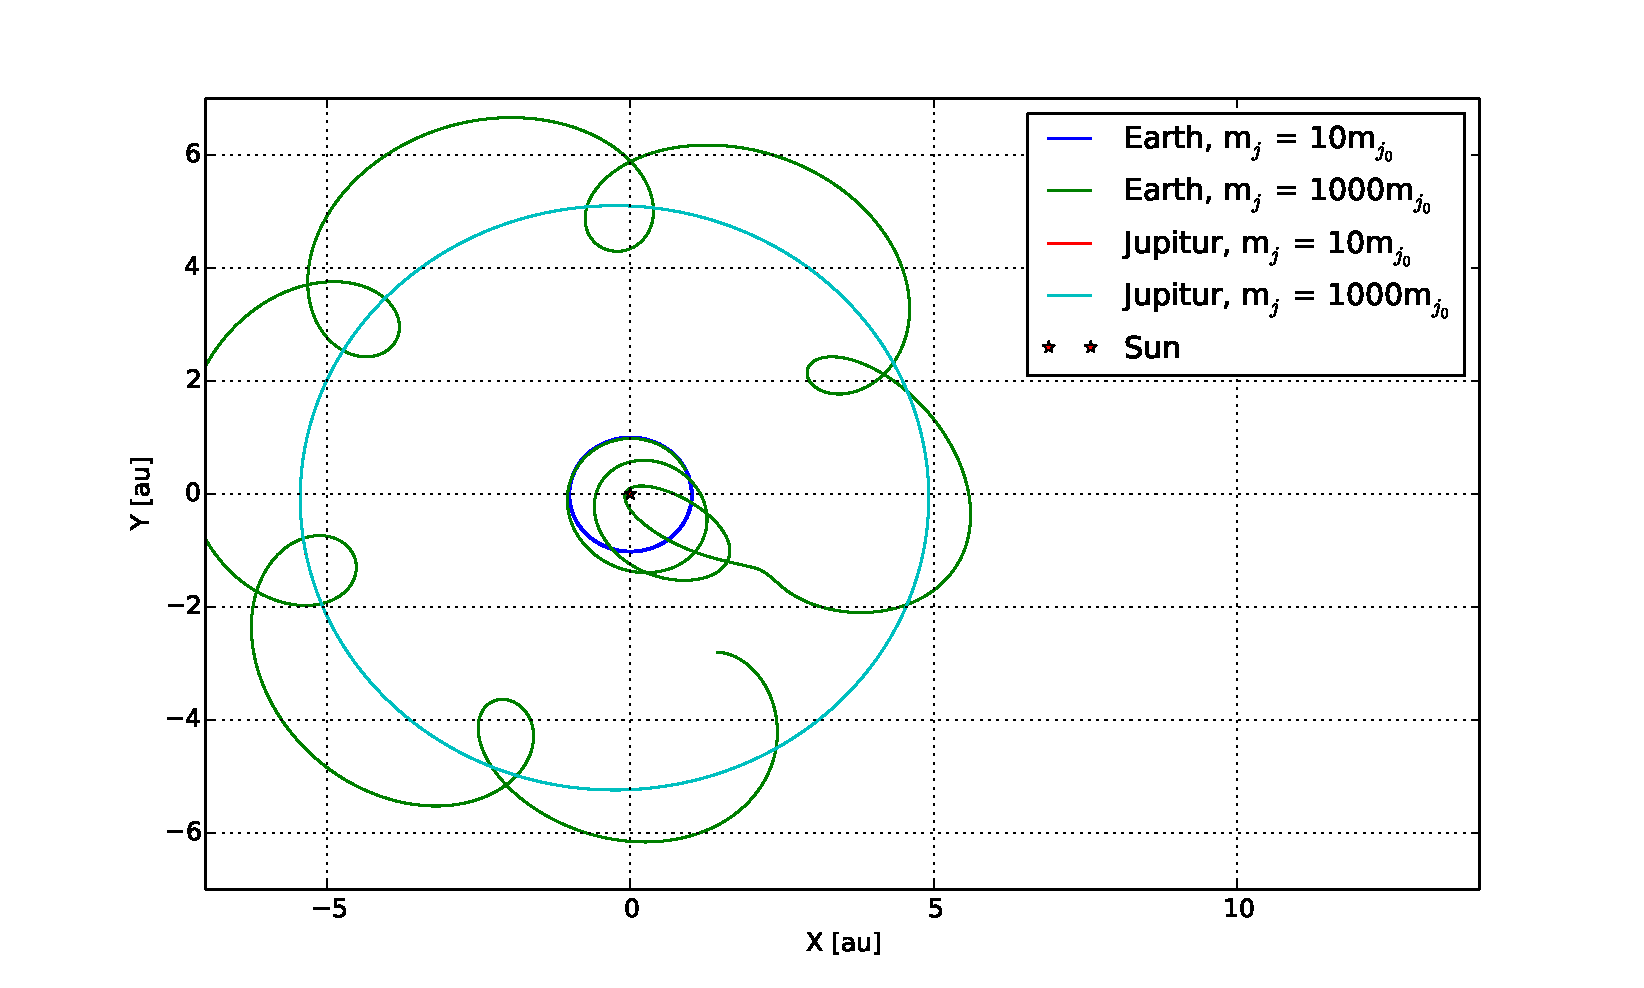
\includegraphics[width=\linewidth]{result/bilder/jupitur-mass-two.pdf}
        \caption{}
    \end{subfigure}
    \caption{Both plot has the sun as a fixed point. What the graphs represent is discussed above and legend should be pretty self explanatory.}
    \label{fig:three-body-varying}
\end{figure}











\subsection{Solar system}

All the figures in this section was made from the results and python scripts in the directory \href{https://github.com/erikfsk/Project-3/tree/master/Project3/full-solarsystem}{\textcolor{blue}{full-solarsystem}}.

\subsubsection{Three planets and all moving}

\begin{figure}[H]
    \centering
    \begin{subfigure}{0.5\textwidth}
        \centering
        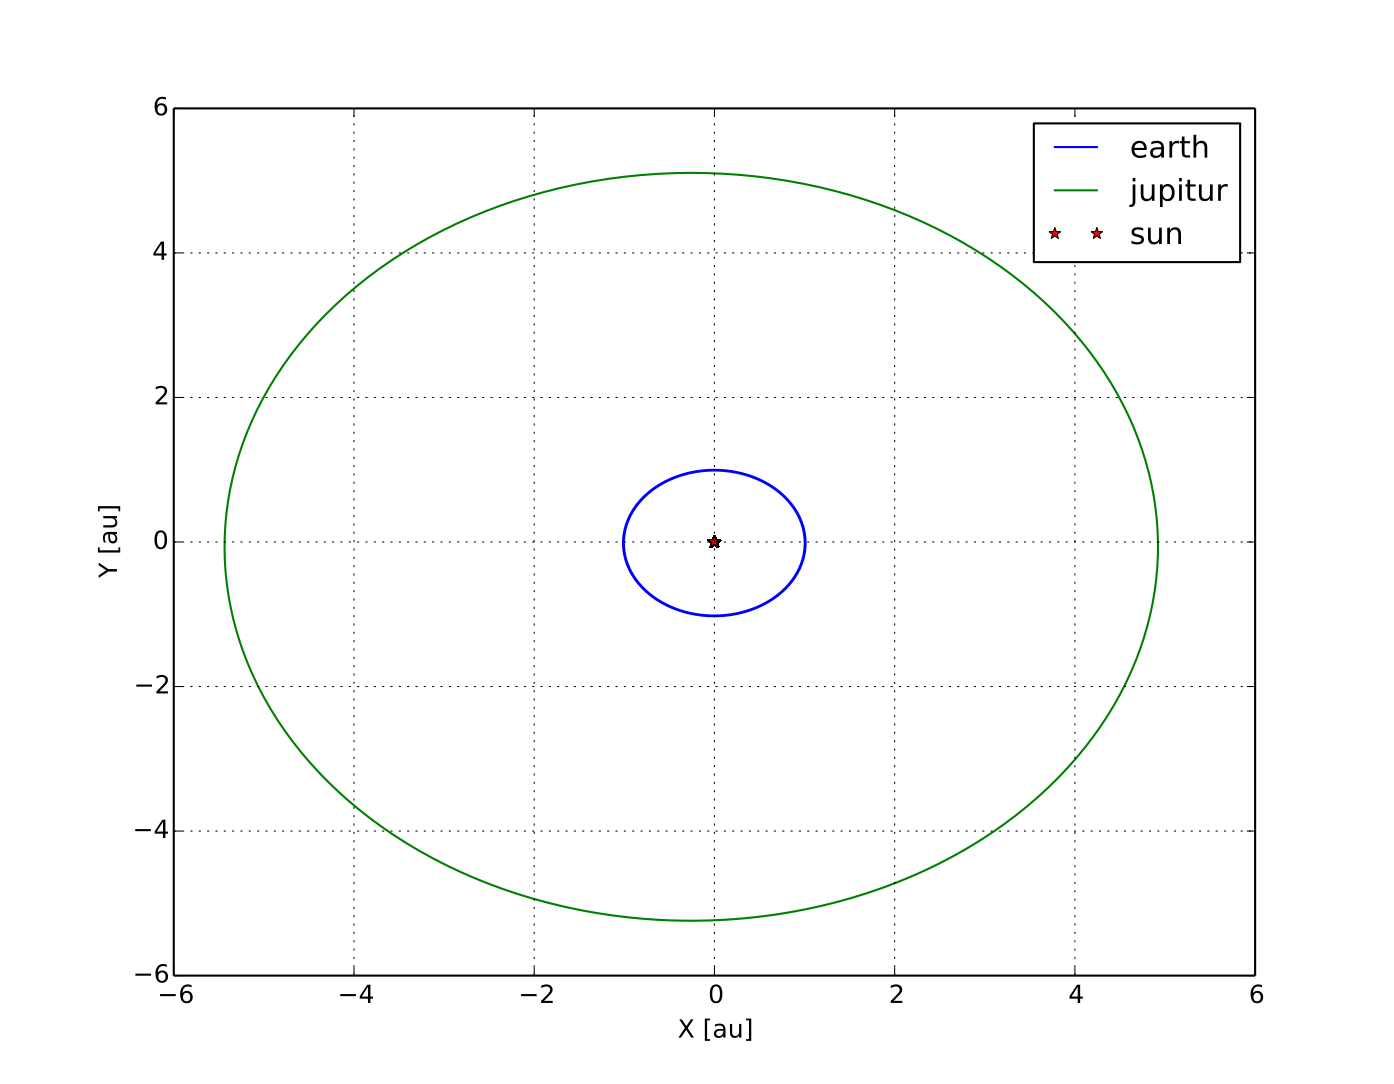
\includegraphics[width=\linewidth]{result/bilder/all-moving-jupitur.png}
        \caption{}
    \end{subfigure}%
    ~ 
    \begin{subfigure}{0.5\textwidth}
        \centering
        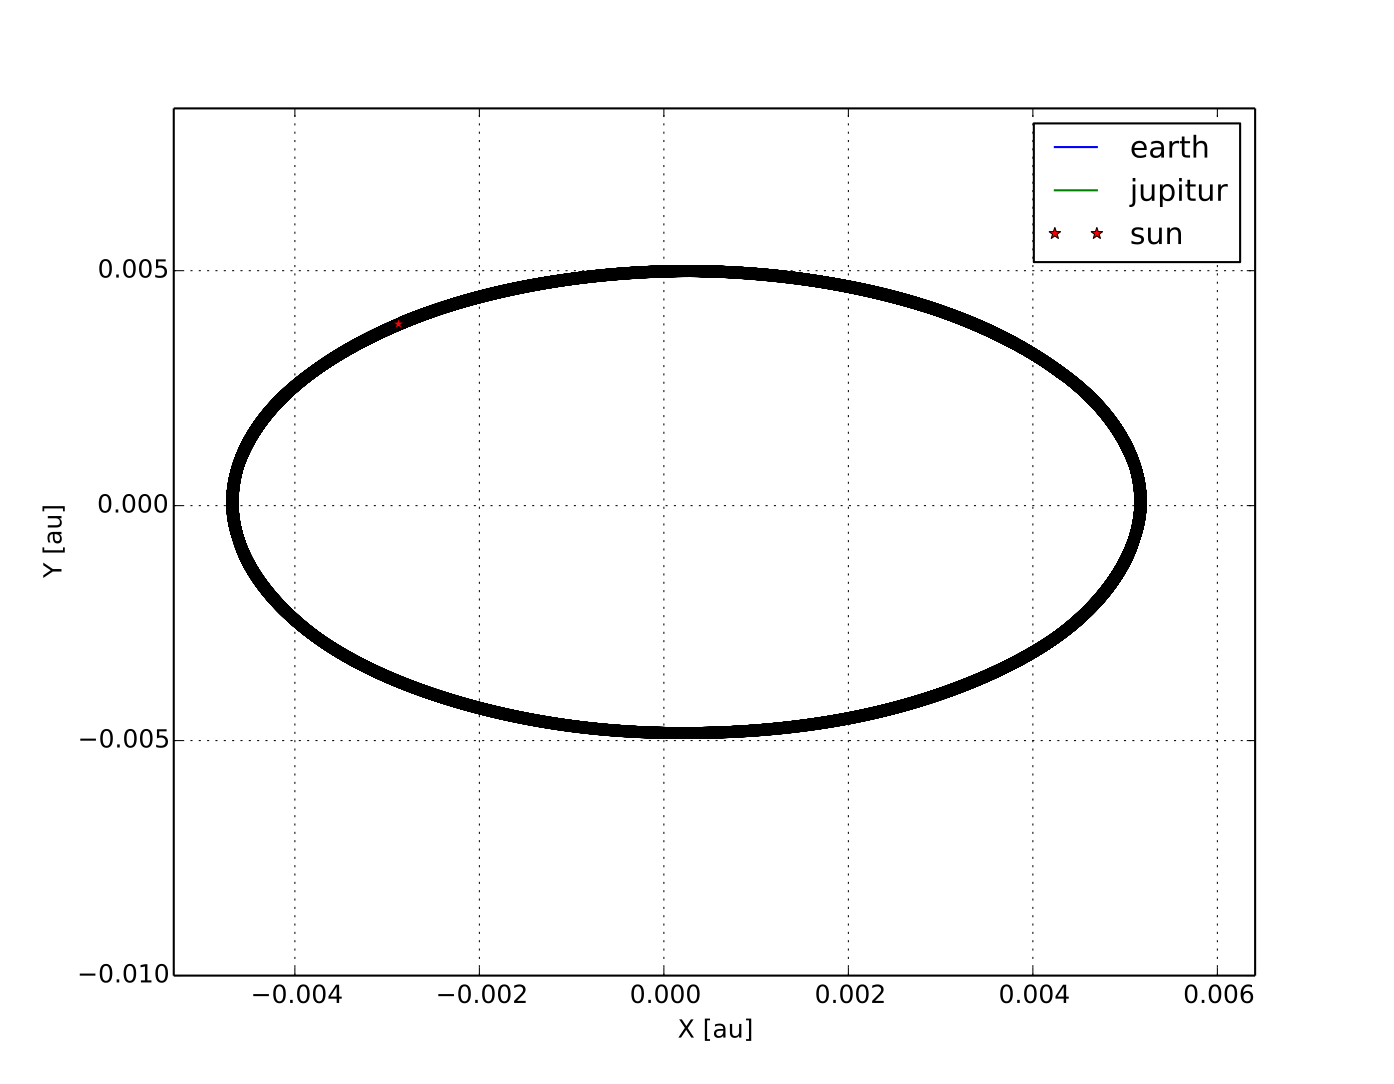
\includegraphics[width=\linewidth]{result/bilder/all-moving-jupitur-mass-center.png}
        \caption{}
    \end{subfigure}
    \caption{a) Shows the three body system solved with a moving sun. It has a n=$10^5$ and ran for 15 years. If this would be used for any tests I would recommend using more points. To use more points here would be stupid. You can't see the difference. b) is a zoom of the middle part of a). This is for verifying that the sun moves around the center of mass and is not drifting.}
    \label{fig:three-body-moving}
\end{figure}

\subsubsection{Solar system all moving}

\begin{figure}[H]
    \centering
    \begin{subfigure}{0.5\textwidth}
        \centering
        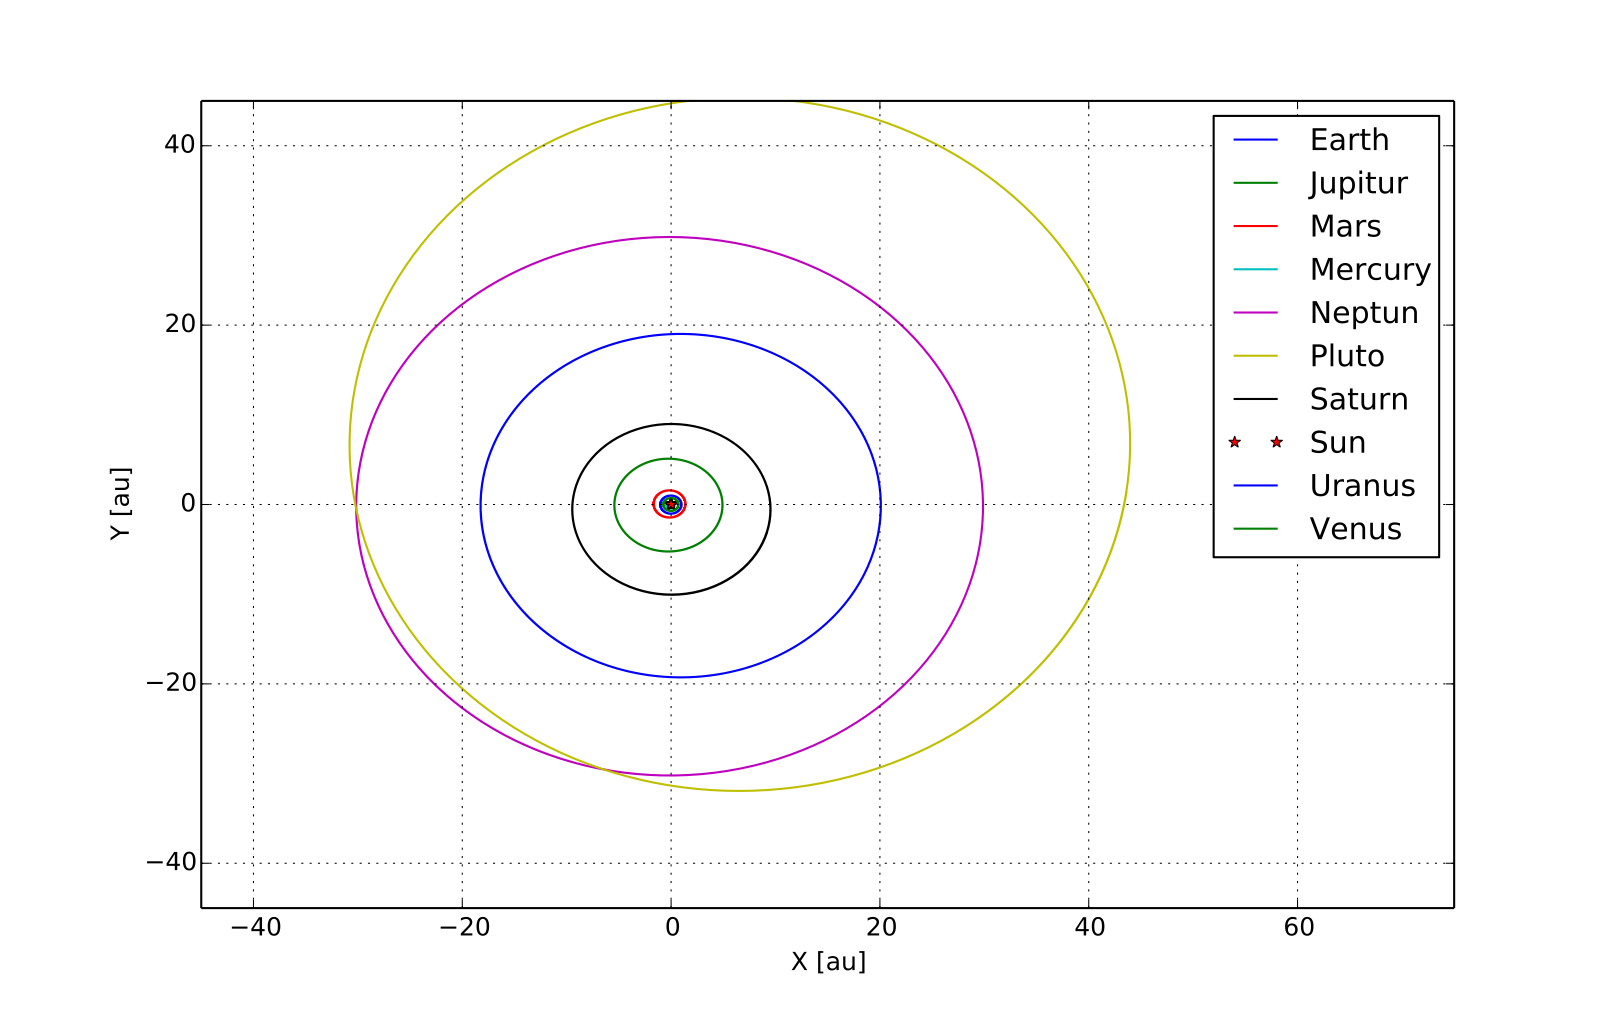
\includegraphics[width=\linewidth]{result/bilder/all-moving-solarsystem.png}
        \caption{}
    \end{subfigure}%
    ~ 
    \begin{subfigure}{0.5\textwidth}
        \centering
        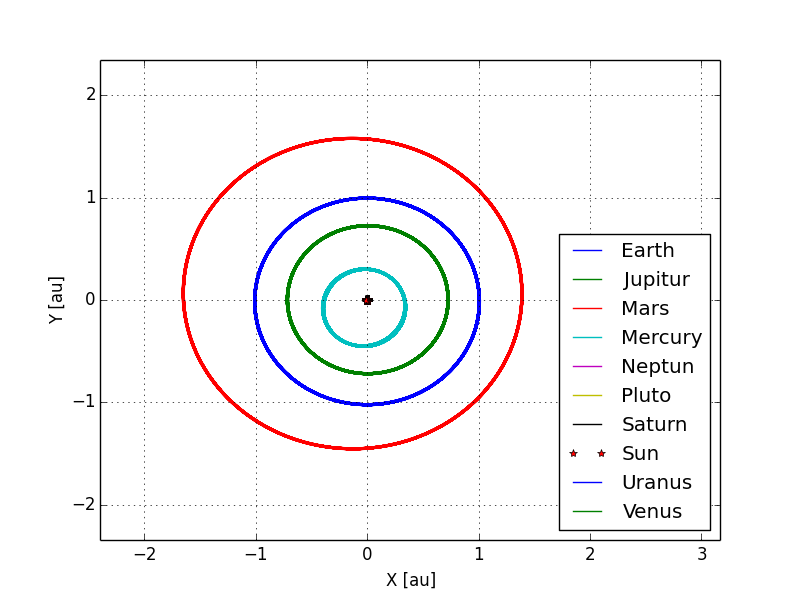
\includegraphics[width=\linewidth]{result/bilder/all-moving-solarsystem-zoom.png}
        \caption{}
    \end{subfigure}
    \caption{a) Shows the hole solar system solved with a moving sun. It has a n=$10^6$ and ran for 300 years. If this would be used for any tests I would recommend using more points, but this would be stupid for this figure, since you can't see the difference. b) is a zoom of the middle part of a). This is so you can see that they also move in orbits.}
    \label{fig:solarsystem-moving}
\end{figure}



\subsection{The perihelion precession of Mercury}

This has been discussed in section \ref{sec:perihelion}. The figure in this section was made from the results and python script in the directory \href{https://github.com/erikfsk/Project-3/tree/master/Project3/mercury-perihelion}{\textcolor{blue}{mercury-perihelion}}.


\begin{figure}[H]
    \centering
    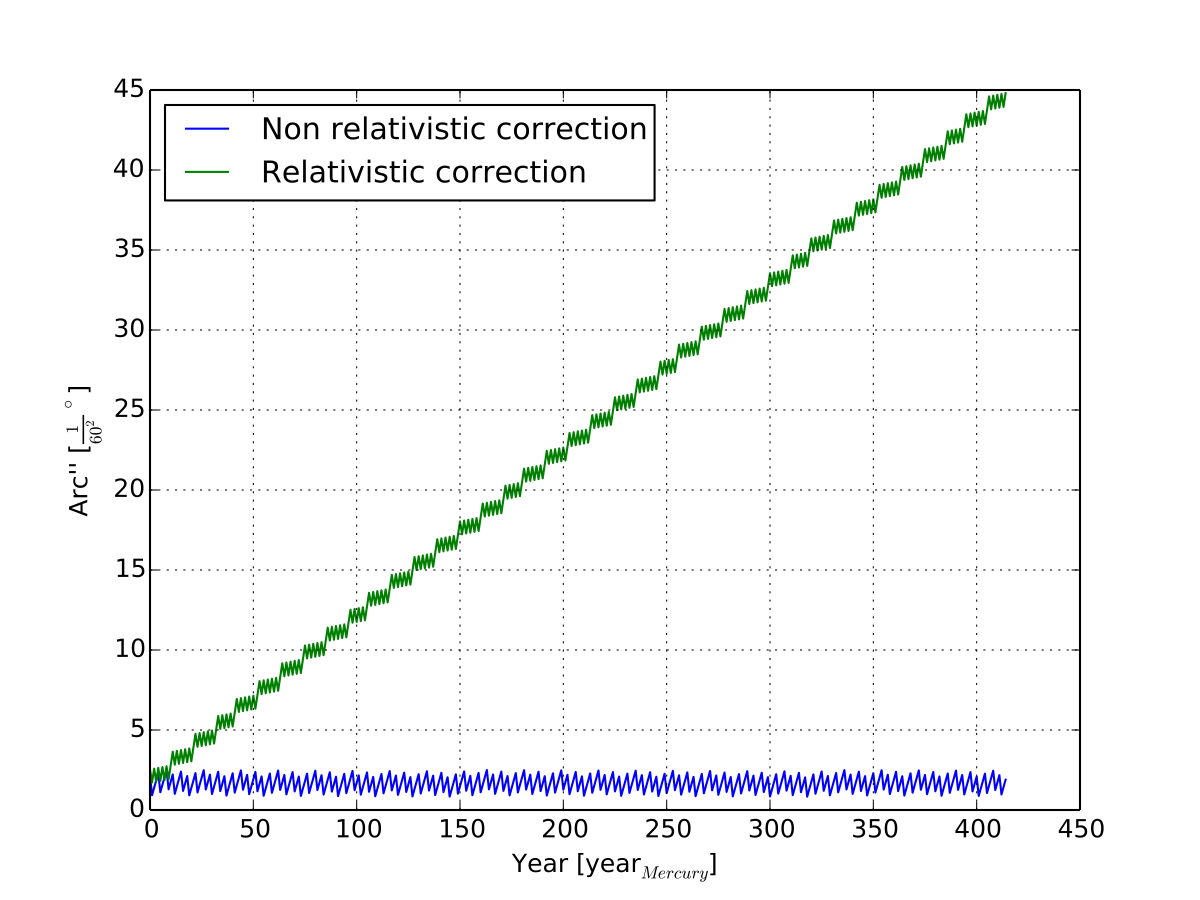
\includegraphics[width=\linewidth]{result/bilder/perihelion.png}
    \caption{The assignment stated that after 100 years mercury perihelion should move about 43''. From the graphs we can see that it should move about 45''. This is probably duo to numerical inaccuracy. The slope's inaccuracy is proably caused by the numerical solver precision. In other words more points would increase the accuracy. The jumping up and down along the linear curve is probably duo to the computer's accuracy with numbers. This will also improve by more steps, but one of them might stop to improve before the other.}
    \label{fig:perihelion}
\end{figure}










%\pagebreak
%\section{Discussion}
%\input{discussion/discussion}


\section{Conclusion}
Both method has been tested and the Verlet-Velocity method comes out as the best. The time is nearly the same, but the Verlet-Velocity conserves energies, momentum and angular momentum for the earth-sun system. After this different scenarios has been studied.  With mostly expected results. The most unexpected result was with the three body system when jupitur had the same mass as the sun. Here the Verlet-Velocity method struggle to produce reasonable results. The relativistic effect on mercury was studied and we are happy to report that our results correspond to observed values\cite{project3}.

Future work should be to get an adaptive step size for the solver. This would probably help the three-body system. It would also be nice if an simple interface was developed, so we dont need to hard code each test. 



\pagebreak
\addcontentsline{toc}{section}{References}
\printbibliography

\pagebreak
\section{Appendix}\label{sec:appendix}
\begin{lstlisting}[language=c++]
//FLOPs FOR ACCELERATION
// 1 FLOP * 3 directions
dx = x1 - x2
// 3 FLOPs
double r = sqrt(dx*dx + dy*dy + dz*dz)
// 7 FLOPs
double a = - (Gconst*m*M/(r*r)) / (m*r)
// 2 FLOPs * 3 directions
a = a + a*(x1-x2);																	
//TOTAL FLOPs = 19 FLOPs 


//FLOPs FOR POSITION :: EULER
// 2 FLOPs * 3 directions
x = x + t_step*Vx															
//TOTAL FLOPs = 6 FLOPs 


//FLOPs FOR VELOCITY :: EULER
// 2 FLOPs * 3 directions
Vx = Vx + t_step*ax															
//TOTAL FLOPs = 6 FLOPs 


//FLOPs FOR POSITION :: Verlet
// 6 FLOPs * 3 directions
x = x + t_step*Vx + (0.5*t_step*t_step*a);
//TOTAL FLOPs = 21 FLOPs


//FLOPs FOR VELOCITY :: Verlet
// 4 FLOPs * 3 directions
Vx = Vx + (0.5*t_step*(Ax+Ax_old));
//TOTAL FLOPs = 12 FLOPs
\end{lstlisting}



%\begin{align*}
%&n \qquad &2^n - (-1)^n\\
%&n+1 \qquad &2^{n+1} - (-1)^{n+1} \\
%& &= 2(2^{n}) - (-1)^{n+1}\\
%& &= 2(2^{n} + (-1)^n  + (-1)^{n+1}) - (-1)^{n+1}\\
%& &= 2(2^{n} + (-1)^n  - (-1)^{n}) - (-1)^{n+1}\\
%& &= 2(2^{n}- (-1)^{n}) + 2(-1)^n  + (-1)^{n}\\
%& &= 2(2^{n}- (-1)^{n}) + 3(-1)^n \\
%\end{align*}



%\begin{tabular}{|c|c|c|c|c|c|c|}
%	\hline 
%	n & General & Specific & LU & fastest & slowest & $\frac{slowest}{fastest}$\\ 
%	\hline
%	10 & 6.5e-05 & 5e-06 & 4e-05 & Specific & General & 13.0\\ 
%	\hline 
%	100 & 7.5e-05 & 8e-06 & 0.0023 & Specific & LU & 287.5\\ 
%	\hline 
%	1000 & 0.00014 & 4e-05 & 0.26 & Specific & LU & 6500\\ 
%	\hline
%	10000 & 0.0007 & 0.0005 & 142.5 & Specific & LU & 285000 \\ 
%	\hline
%\end{tabular}

%\begin{figure}[H]
%		\centering
%		\includegraphics[width=0.7\linewidth]{ab.png}
%		\caption{Atomene er gule kuler, de elementære vektorene er blå og a vektorene er grønne.}
%		\label{fig:ab}
%\end{figure}



\end{document}
